\documentclass[border=2mm]{standalone}
\setlength{\textwidth}{12.2cm}
\setlength{\textheight}{19.3cm}
\usepackage{pgfplots}
\usepgfplotslibrary{statistics}
\pgfplotsset{compat=1.8}

% \renewcommand{\scalefont}[1]{\small}

\begin{document}
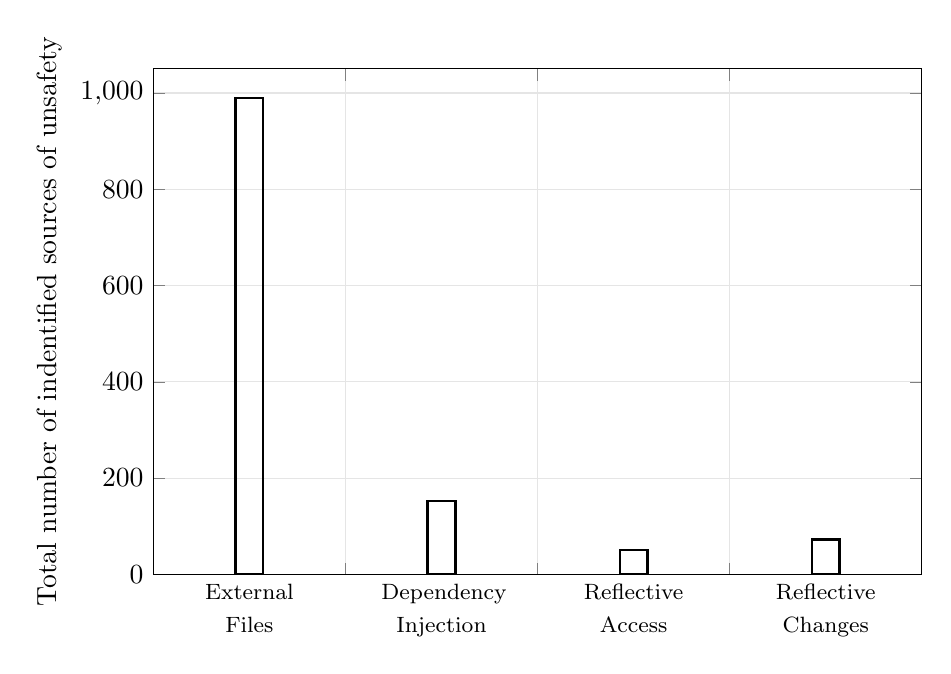
\begin{tikzpicture}
    \begin{axis}[
            ybar,
            color={black},
            ylabel={Total number of indentified sources of unsafety},
            height=8cm,
            grid=both,
            grid style={gray!20},
            ymin=0,ymax=1050,
            % ytick={0,10,...,75},
            x=\textwidth/5,xmin=0,xmax=4,
            xtick={0,1,2,...,4},
            x tick label as interval,
            xticklabels={
                    \footnotesize{External Files},
                    \footnotesize{Dependency Injection},
                    \footnotesize{Reflective Access},
                    \footnotesize{Reflective Changes}
                },
            x tick label style={
                    text width=\textwidth/8,
                    align=center
                },
            xtick align=inside,
        ]
        % DATA:
        % 10000 Commits, 1151 detected commits with one source of unsafety, counted multiple times for
        % multiple unsafeties. Percentages rounded to two decimal places
        % 989 External Files -> 989 / 1151 * 100 -> 85.93
        % 153 Dependency Injection -> 153 / 1151 * 100 -> 13.29
        % 51 Reflection Access -> 51 / 1151 * 100 -> 4.43
        % 72 Reflection Changes -> 72 / 1151 * 100 -> 6.26
        % \pie[color={black!10, black!20, black!30, black!40},text=pin]{
        %     85.93/External Files,
        %     13.29/Dependency Injection,
        %     4.43/Reflection Access,
        %     6.26/Reflection Changes
        % }
        \addplot[draw=black, line width=0.3mm] coordinates {
                (0.5, 989)
                (1.5, 153)
                (2.5, 51)
                (3.5, 72)
            };
    \end{axis}
\end{tikzpicture}
\end{document}
